% !TeX root=main.tex
\chapter{فشرده‌سازی شبکه 
\lr{LXMERT}
}
\thispagestyle{empty}
\iffalse
هدف این پروژه بررسی صحت فرضیه بلیت برنده
\LTRfootnote{\lr{lottery ticket hypothesis}}
بر شبکه
\lr{LXMERT}
می‌باشد. همچنین دو روش دیگر هرس شامل هرس اتصالات به صورت تصادفی
\LTRfootnote{\lr{random pruning}}
و هرس اتصالات با وزن زیاد
\LTRfootnote{\lr{high magnitude pruning}}
مورد بررسی قرار می‌گیرد.
\fi
\iffalse
\section{فشرده‌سازی شبکه 
\lr{LXMERT}
}
\fi
در این پژوهش به سه روش فشرده‌سازی (هرس) شبکه
\lr{LXMERT}
انجام شده و تلاش برای یافتن بهترین روش فشرده‌سازی صورت گرفته است. هر سه روش هرس بر پایه وزن اتصالات می‌باشند. بررسی نتایج و تاثیر هرس بر دقت شبکه بر روی مجموعه داده
\href{https://visualqa.org/download.html}{\lr{VQA v2.0}}
بررسی شده است. در اجرا از مقادیر از پیش تعیین شده ابرپارامتر‌ها 
\LTRfootnote{\lr{Hyperparameters}}
در شبکه
\lr{LXMERT}
استفاده شده است. 
\newline
به جز اتصالات embedding ورودی و اتصالات لایه خروجی، برای سایر اتصالات احتمال حذف شدن وجود دارد. این روش‌ها از میزان هرس 10 درصد شبکه تا هرس 90 درصد شبکه در سه 
\lr{seed}
تکرار شد؛ تا علاوه بر بررسی تاثیر نوع و میزان حذف اتصالات بر دقت نهایی، با تکرار در سه   
\lr{seed}
میزان قابل اطمینان بودن نتایج به دست‌آمده مورد بررسی قرار گیرد.
\newpage
\section{هرس اتصالات کم وزن}\label{LOWMagnitude}
	
این روش همانند فرضیه بلیط بخت‌آزمایی
\LTRfootnote{\lr{Lottery Ticket Hypothesis}}
می‌باشد. صحت این فرضیه تا به حال در شبکه‌های کاملا متصل و شبکه پیچشی مورد بررسی قرار گرفته است. حال قرار است صحت آن بر یک ترنسفورمر زبانی-تصویری دو جریانه
\LTRfootnote{\lr{cross-modal}}
 مورد بررسی قرار دهیم.
در این روش به صورت هرس تکرارشونده
\LTRfootnote{\lr{Iterative Pruning}}
عمل شد. مراحل الگوریتم به صورت زیر می‌باشد.
\begin{enumerate}
	\item وزن‌های از قبل آموزش دیده مدل
	\lr{LXMERT}
	به همراه رده‌بند
	\lr{VQA}
	به شبکه داده می‌شود. این مقادیر برای مراحل بعد ذخیره می‌شود.
	\item مدل بر روی 3129 جواب پرتکرار مجموعه داده
	\lr{VQA v2.0}
	آموزش می‌بیند. آموزش  4 بار تکرار
	\LTRfootnote{\lr{Iteration}}
	می‌شود. در نهایت مدل
	\lr{finetune}
	شده بر روی مسئله
	\lr{VQA}
 به دست می‌آید.	مقادیر دقت به دست‌آمده از این مرحله با برچسب
 \lr{Unpruned Badeline}
 در نمودار‌ مشاهده می‌شود.
	\item
	در این مرحله هر بار 10 درصد از اتصالات کم‌وزن شبکه به صورت تکرار شونده حذف می‌شود. این مرحله تا زمانی که درصد مشخصی از کل اتصالات شبکه حذف شود ادامه پیدا می‌کند. برای همه اتصالات به جز اتصالات لایه 
	\lr{embedding}
	و اتصالات لایه خروجی، احتمال حذف در این مرحله وجود دارد. پس از رسیدن به درصد هرس مشخص، دقت شبکه هرس شده بر روی مجموعه داده 
	\lr{VQA}
	با برچسب 
	\lr{pruned}
	در نمودار مشخص می‌شود.
	\item پس حذف مقدار مشخصی از اتصالات (اتمام هرس) وزن‌های ذخیره شده در مرحله اول به شبکه بازنشانی
	\LTRfootnote{\lr{Reset}}
	 می‌شود. مقادیر دقت به دست‌آمده از این مرحله با برچسب
	\lr{reset initial weight}
	در نمودار‌ مشاهده می‌شود.
	\item حال شبکه هرس شده به تعداد تکرار مشابه مرحله 2 آموزش می‌بیند. در نهایت دقت شبکه در این حالت بررسی می‌شود. مقادیر دقت به دست‌آمده از این مرحله با برچسب
	\lr{retrain}
	در نمودار‌ مشاهده می‌شود.
\end{enumerate}

نتایج هرس اتصالات کم‌وزن شبکه
\lr{LXMERT}
 در نمودار شکل \ref{low_pruning} قابل مشاهده است.

لازم به ذکر است همه دقت‌های گزارش شده، از ارزیابی بر روی مجموعه داده 
\lr{Test\_dev (Validaion)}
به دست آمده است.

\begin{figure}[H]
	\center{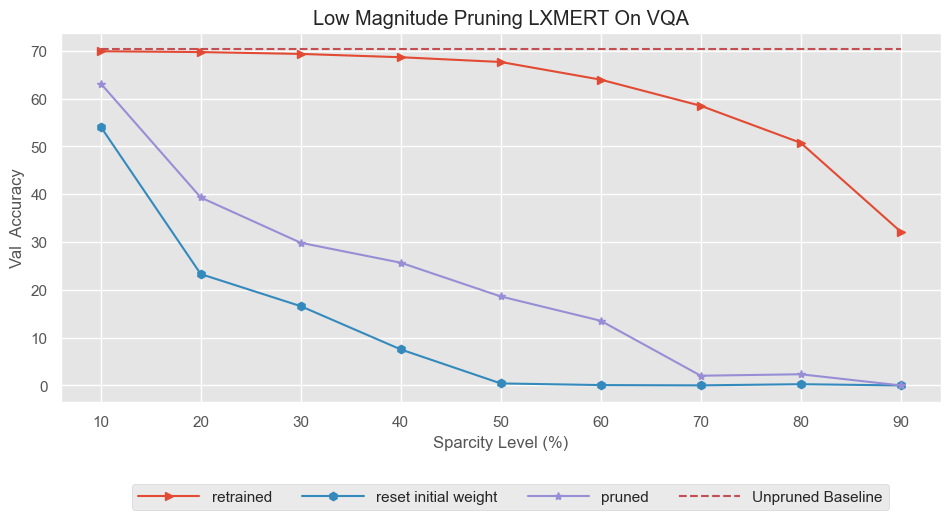
\includegraphics[width=0.9\linewidth]{images/Low_Magnitude_experiment_result.PNG}}
	\caption{نتایج حاصل از هرس اتصالات کم‌وزن}
	\label{low_pruning}
\end{figure}



\subsection{تحلیل نتایج}
از آزمایش‌های انجام شده این نتیجه حاصل می‌شود که می‌توان 50 تا 60 درصد اتصالات کم‌وزن شبکه 
\lr{LXMERT}
را بدون کاهش شدیدی در دقت نهایی حذف کرد. این نتیجه نمایان‌گر آن است که 50 درصد اتصالات عملا تاثیری چندانی ندارند و قابل حذف هستند. همچنین فرضیه بلیط بخت‌آزمایی در شبکه دو جریانه
\lr{LXMERT}
برقرار است.
همان‌طور که از نمودار‌های رسم شده مشخص است، همه نمودار‌ها روند نزولی دارند. به این صورت که هر چه تعداد بیشتری از اتصالات را حذف کنیم، دقت شبکه کاهش پیدا می‌کند. اگر میزان حدف اتصالات بیش از 50 درصد باشد، شاهد کاهش دقت شدیدتری هستیم.
\newline
همچنین نتایج نشان می‌دهد اتصالات کم‌وزن در شبکه عصبی تاثیر کمتری در کارایی نهایی شبکه دارند. بنابراین اگر نصف اتصالات کم‌وزن حذف شود تاثیر چندانی در دقت نهایی ندارد. پس آموزش اتصالات و مقدار وزن آن‌ها به بهترین شکل صورت گرفته و وزن اتصالات نشان‌دهنده اهمیت آن‌ها می‌باشد.

\section{هرس اتصالات به صورت تصادفی}

	در این روش به صورت کاملا تصادفی تعدادی از وزن‌های شبکه را حذف کرده و سایر اتصالات باقی‌مانده را نگه می‌داریم. نتایج هرس اتصالات شبکه
	\lr{LXMERT}
	به صورت تصادفی در نمودار شکل \ref{random_pruning} قابل مشاهده است.
	
	
\begin{figure}[H]		  		    \center{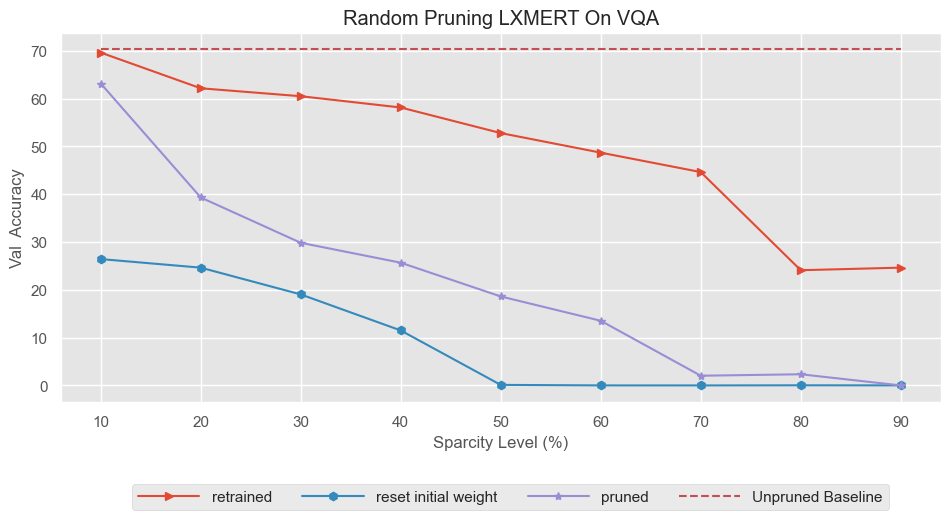
\includegraphics[width=0.9\linewidth]{images/Random_experiment_result.PNG}}
	\caption{نتایج حاصل از هرس اتصالات به صورت تصاذفی}
	\label{random_pruning}
\end{figure}
\subsection{تحلیل نتایج}	
همچون شکل \ref{low_pruning} که نتایج قسمت \ref{LOWMagnitude} را نشان می‌دهد، در این قسمت نیز نمودار نزولی داریم (شکل \ref{random_pruning}). به این صورت که با افزایش میزان هرس شبکه، دقت نیز به همان نسبت کاهش پیدا می‌کند. با توجه به اینکه در این حالت اتصالات تصادفی انتخاب می‌شوند از میزان هرس 20 درصد و بیشتر کاهش دقت بیشتری رخ می‌دهد. پس می‌توان به این صورت مطرح کرد که اتصالاتی که وزن کمتری دارند، تاثیر کمتری در دقت نهایی شبکه داشتند. به همین علت بود که در هرس اتصالات کم وزن(قسمت \ref{LOWMagnitude}) با حذف 50 درصد اتصالات کم وزن دقت تغییر چشم‌گیری نداشت.

\section{هرس اتصالات با وزن زیاد}\label{high_mag_pruning}

در این روش اتصالاتی که در هرس 
\ref{LOWMagnitude}
نجات یافته‌اند، حذف می‌شوند. به عبارت دیگر در این روش اتصالات با وزن زیاد حذف می‌شوند. نتایج حاصل از اجرا در شکل
\ref{high-mag}
قابل مشاهده است.

\begin{figure}[H]
	\center{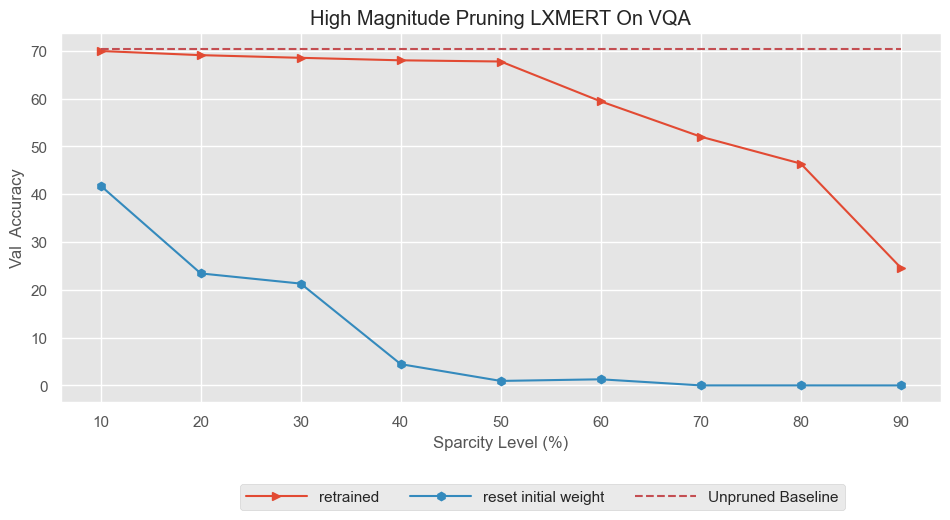
\includegraphics[width=0.9\linewidth]{images/High_Magnitude_experiment_result.PNG}}
	\caption{نتایج حاصل از هرس اتصالات با وزن زیاد}
	\label{high-mag}
\end{figure}
\subsection{تحلیل نتایج}
همان‌طور که در شکل
\ref{high-mag}
مشاهده می‌شود، با افزایش میزان حذف اتصالات دقت نهایی شبکه کاهش می‌یابد. شیب نمودار از نمودار
\ref{low_pruning}
تندتر است بدین معنی که تغییرات با شدت بیشتری رخ داده است. انتظار می‌رفت تغییرات نمودار و دقت نهایی از دو بخش قبل بدتر باشد ولی نتایج به دست‌آمده با پیش‌بینی‌ها مغایرت دارد.
\newpage
\section{مقایسه نتایج}
در شکل \ref{ex_result} خلاصه نتایج سه نوع هرس معرفی شده به تفکیک میزان هرس و بر اساس نوع هرس قابل مشاهده است. همچنین در جدول \ref{res_all} اعداد دقیق برای بررسی‌های احتمالی گزارش شده است.
\begin{table}[ht]
	\caption{نتایج مدل هرس‌شده آموزش دیده برای انواع هرس به تفکیک درصد حذف اتصالات}
	\label{res_all}
	\centering
	\onehalfspacing
	\begin{tabular}{|c|c|c|c|}
		\hline درصد هرس & اتصالات با وزن کم &  اتصالات تصادفی & اتصالات با وزن زیاد\\ 
		\hline 10 & $69.94 \pm 0.03$ & $69.58 \pm 0.02$  &  $69.75 \pm 0.13$\\ 
		\hline 20 & $69.59 \pm 0.11$ & $62.21 \pm 0.06$  &  $69.17 \pm 0.09$\\ 
		\hline 30 & $69.23 \pm 0.07$ & $60.23 \pm 0.24$  &  $68.60 \pm 0.08$\\ 
		\hline 40 & $68.70 \pm 0.05$ & $57.49 \pm 0.62$  &  $67.87 \pm 0.18$\\ 
		\hline 50 & $67.44 \pm 0.14$ & $52.63 \pm 0.13$  &  $67.78 \pm 0.04$\\ 
		\hline 60 & $63.94 \pm 0.01$ & $48.68 \pm 0.00$  &  $58.76 \pm 0.63$\\ 
		\hline 70 & $58.50 \pm 0.04$ & $44.96 \pm 0.34$  &  $52.28 \pm 0.26$\\ 
		\hline 80 & $50.63 \pm 0.21$ & $24.36 \pm 0.26$  &  $46.54 \pm 0.15$\\ 
		\hline 90 & $28.12 \pm 4.02$ & $24.36 \pm 0.26$  &  $25.40 \pm 0.77$\\ 
		\hline 
	\end{tabular} 
\end{table}

\begin{figure}[H]
	\center{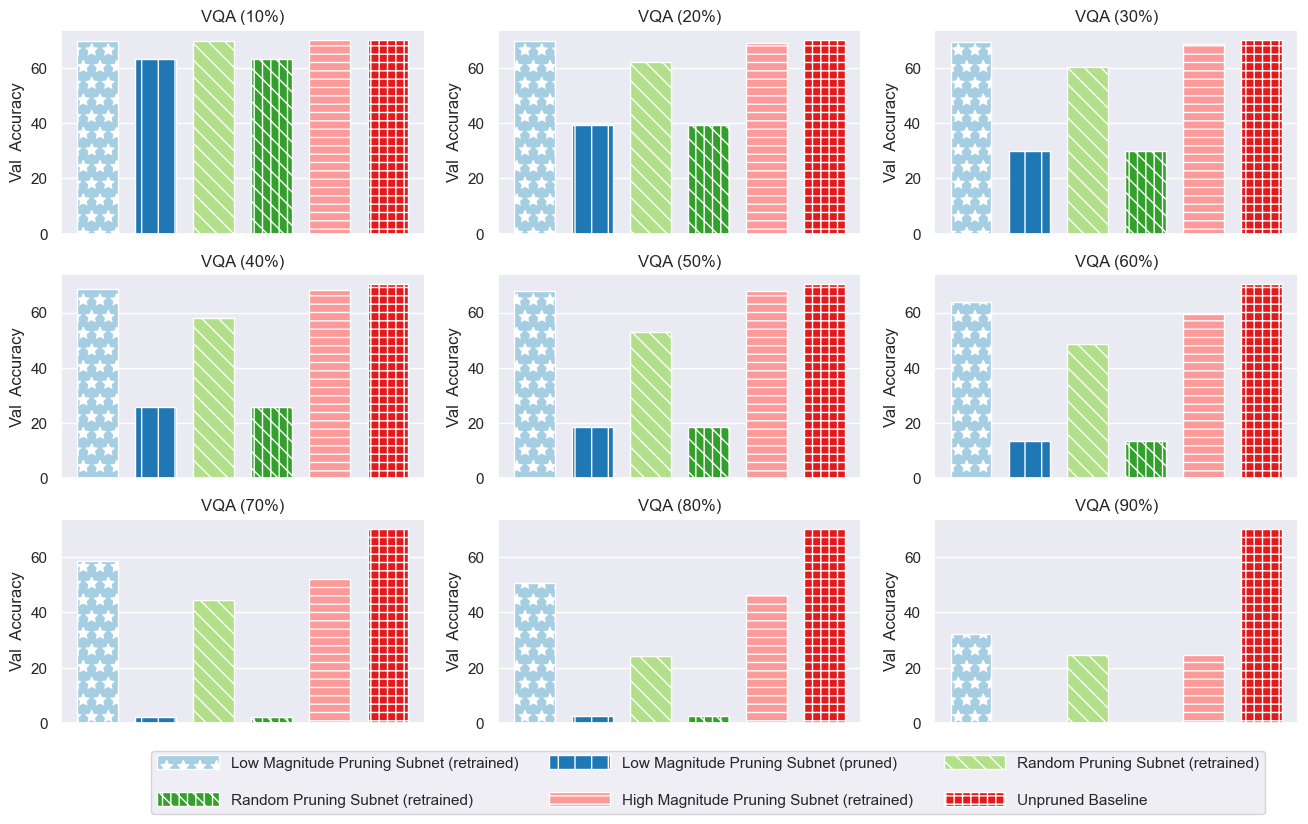
\includegraphics[width=1\linewidth]{images/experiment_result.PNG}}
	\caption{نتایج انواع هرس به تفکیک درصد حذف اتصالات}
	\label{ex_result}
\end{figure}

\newpage
\section{نحوه پیاده‌سازی و اجرا آزمایش‌ها}
پیاده‌سازی پروژه در 
\href{https://github.com/ghazaleh-mahmoodi/LXMERT-Compression}{اینجا}
قابل مشاهده می‌باشد که با زبان پایتون و فریم‌ورک پایتورچ انجام شده است. برای شبکه 
\lr{LXMERT}
از پیاده‌سازی اصلی مقاله و ابر پارامتر‌های تعیین شده که در 
\href{https://github.com/airsplay/lxmert}{گیت‌هاب}
موجود می‌باشد، استفاده شد.
\newline
برای اجرا از سخت‌افزار
\lr{GPU.1080Ti.xlarge}
با رم 
\lr{31.3GB}
استفاه شد. دستور 
\lr{nvidia-smi}
میزان استفاده از 
\lr{GPU}
را نمایش می‌دهد. خروجی این دستور در هنگام اجرا آزمایشات به صورت شکل \ref{nvidia-smi} شد.
\begin{figure}[H]		  		    \center{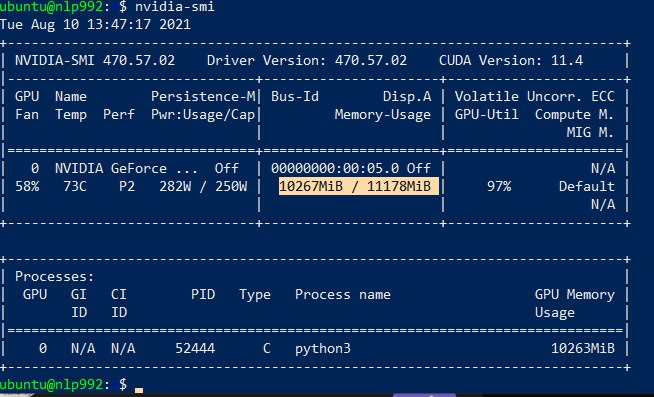
\includegraphics[width=0.7\linewidth]{images/nvidia-smi.jpg}}
	\caption{میزان مصرف
\lr{GPU}	
}
	\label{nvidia-smi}
\end{figure}
هر دوره
\LTRfootnote{\lr{Epoch}}
اجرا نزدیک به 2 ساعت زمان می‌گیرد. فرآیند هرس شبکه هم حدودا نیم ساعت زمان می‌خواهد. تعداد اجرا پیش فرض 4 می‌باشد. بنابراین هر آزمایش شامل فرآیند هرس به میزان مشخص، بازنمایی
\LTRfootnote{\lr{Reset}}
 وزن‌های اولیه و آموزش شبکه هرس شده نزدیک به 9 ساعت زمان می‌گیرد. با توجه به این موضوع برای اجرا آزمایش‌ها کد اتوماتیک نوشته شد که برای 3 
\lr{seed}
به ازای 3 مدل هرس (اتصالات کم‌وزن، تصادفی، اتصالات با وزن زیاد) و برای میزان هرس 10 درصد تا 90 درصد (9 مقدار) به صورت پشت سر هم اجرا شود. به این صورت از منابع 
\lr{GPU}
به بهترین صورت ممکن استفاده شد.
با توجه به سنگین بودن مجموعه داده 
\lr{VQA v2.0}
رم
\lr{GPU}
می‌بایست از 
\lr{6900 MiB}
بیشتر باشد. 
\newline
\newline
برای اجرا آزمایش‌ها لازم است با دستور 
\lr{pip3 install -r requirements.txt}
پکیج‌های مورد نیاز برای اجرا کد را نصب کنید. با توجه به طولانی بودن زمان اجرا کل آزمایش‌ها بهتر است با دستور 
\lr{screen}
یک اسکرین جدید برای اجرا بسازید و به شکل معمول دستورات را اجرا کنید. در این صورت حتی با بستن ترمینال اجرا ادامه پیدا می‌کند. با
\lr{screen -r}
در صورت باز کردن مجدد ترمینال می‌توانید فرآیند و میزان پیش‌رفت اجرا را ببینید.
راه حل دیگر برای تداوم اجرا در صورت بستن ترمینال استفاده از دستور 
\lr{nohup}
است. کافیست
\lr{nohup bash run/vqa\_run.bash}
را اجرا کنید. خروجی‌های اجرا در 
\lr{nohup.out}
قابل مشاهده می‌باشد.
\newline
در صورتی که یک
\lr{screen}
جدید برای خود ساختید، با دستور
\lr{bash run/vqa\_run.bash}
کلیه آزمایش‌ها به صورت متوالی اجرا می‌شود. در نهایت نتایج به دست‌آمده در فایل
\lr{json}
در پوشه 
\lr{result}
ذخیره می‌شود. همچنین
\lr{mask}
های هرس و وزن‌های شبکه در پوشه
\lr{models}
قابل مشاهده می‌باشند. 










